% ==========================================
% Section 1: Introduction (Slides 1-5)
% ==========================================

% Slide 1: Title Slide
\begin{frame}[plain]
  \vspace*{-0.2cm}
  \noindent\begin{minipage}[t]{0.65\textwidth}
    {\fontsize{24}{28}\selectfont\color{mannheimblue}\textbf{پیش‌پردازش داده‌ها}}\\[8pt]
    {\fontsize{15}{18}\selectfont\color{mannheimblue}\lr{IE500} داده‌کاوی}
  \end{minipage}%
  \hfill
  \begin{minipage}[t]{0.30\textwidth}
    \flushleft
    
\includegraphics[height=1.1cm]{images/mannheim_logo.png}
  \end{minipage}

  \vspace{0.6cm}
  \noindent\makebox[\textwidth][c]{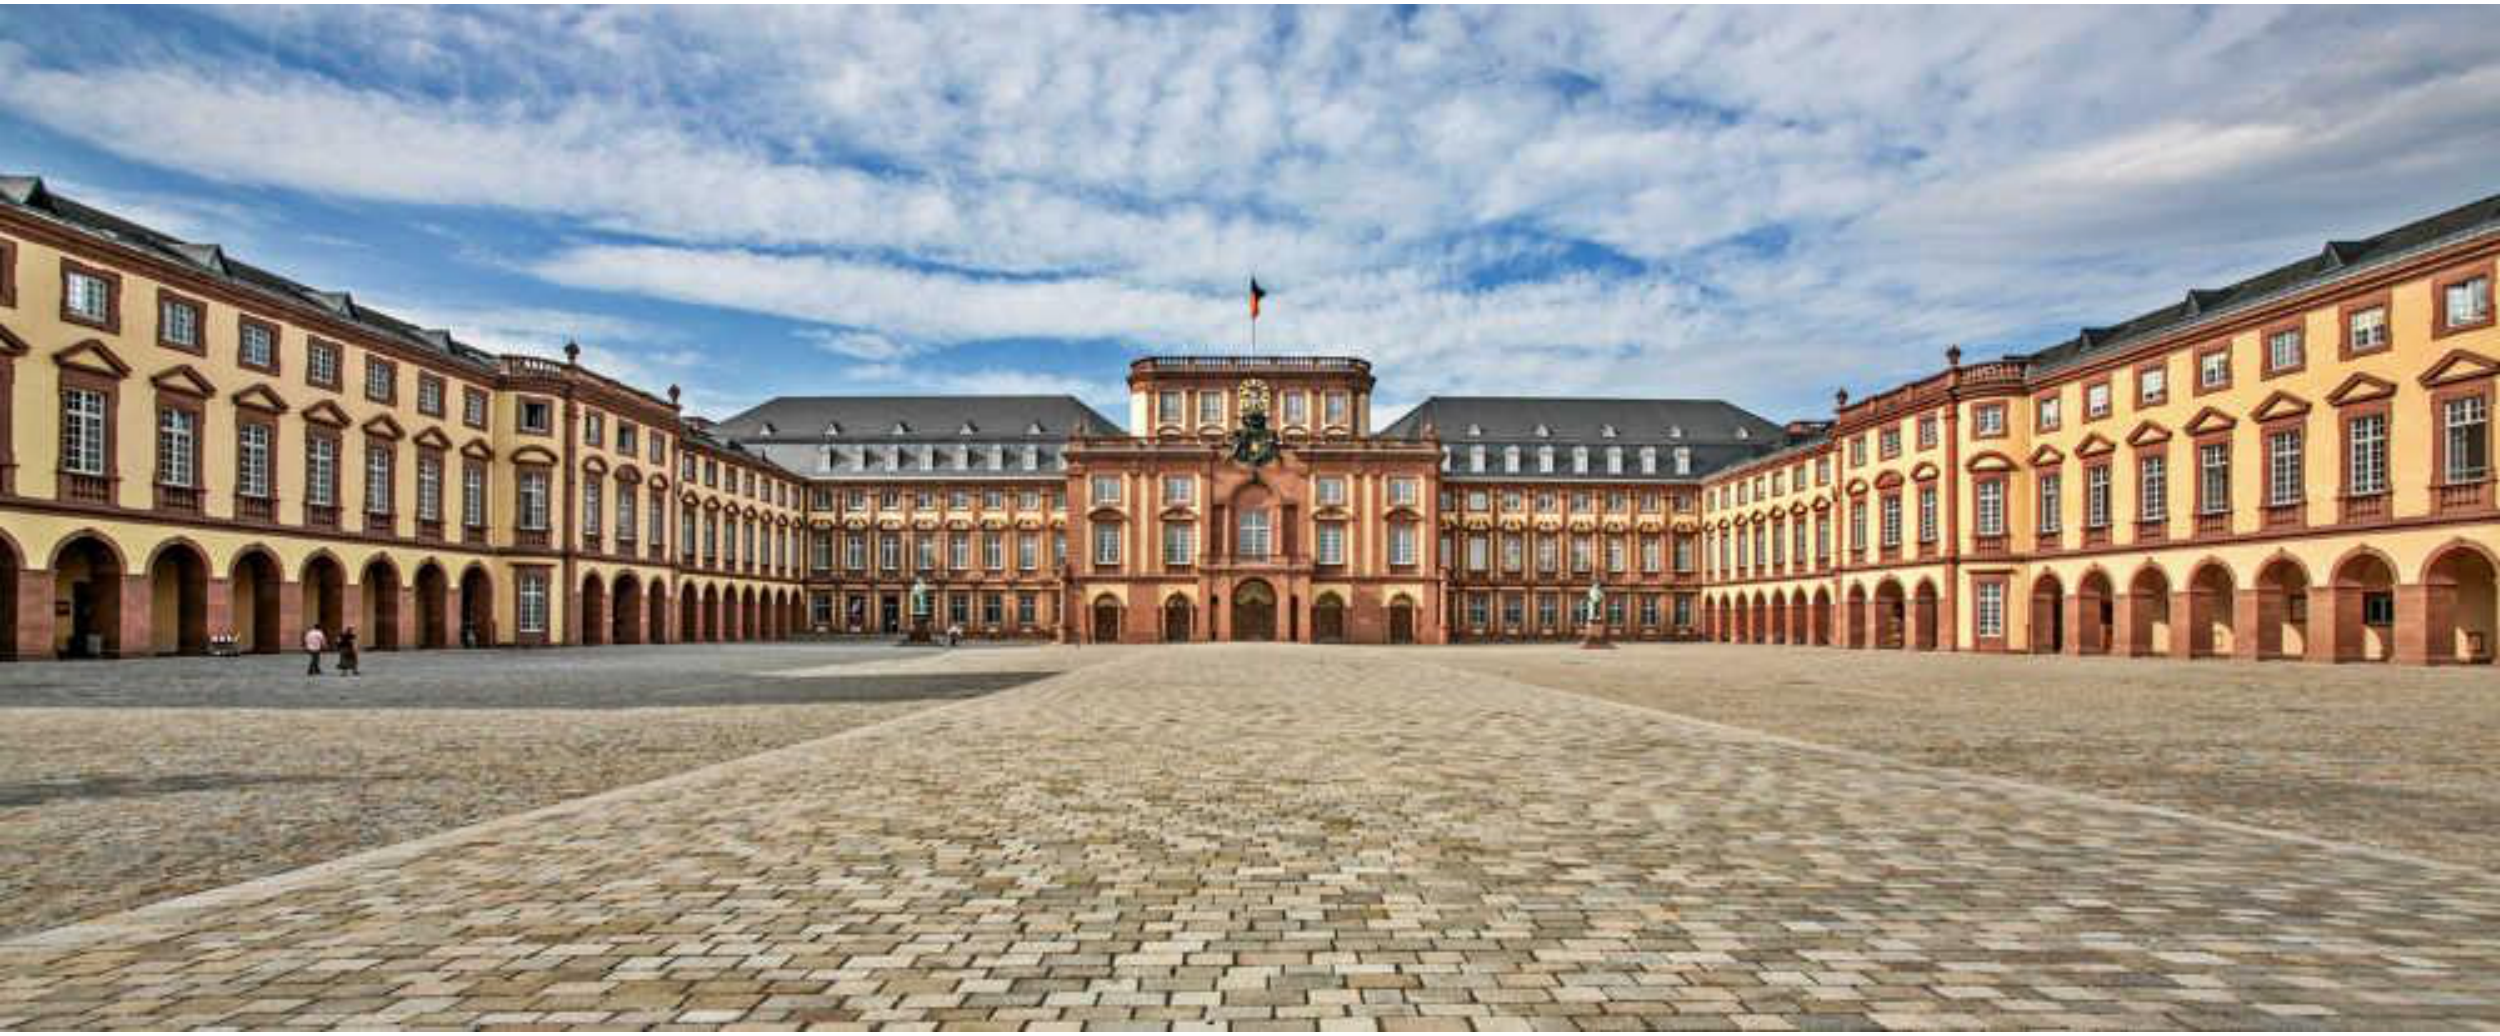
\includegraphics[width=\paperwidth,height=4.8cm]{images/page_01_img_1.png}}

  \vfill
  \leavevmode%
  \hbox to \textwidth{%
    {\fontsize{6.8}{8}\selectfont\color{subgray}دانشگاه مانهایم \ | \ \lr{IE500} داده‌کاوی \ | \ پیش‌پردازش داده‌ها \ | \ نسخه \lr{28.10.2024}}%
    \hfill%
    {\fontsize{7.5}{9}\selectfont\color{subgray}۱}%
  }%
  \vspace*{-0.1cm}
\end{frame}

% Slide 2: Lincoln Quote
\begin{frame}{مقدمه}
\begin{columns}[c]
  \begin{column}{0.62\textwidth}
    \begin{itemize}
      \item \textbf{«به من شش ساعت برای قطع یک درخت فرصت بدهید، چهار ساعت اول را صرف تیز کردن تبر خواهم کرد.»}
    \end{itemize}
    \vspace{1.6cm}
    \flushleft
    {\fontsize{10}{12}\selectfont\color{mannheimblue}\textbf{آبراهام لینکلن} (\lr{1809--1865})}
  \end{column}
  \begin{column}{0.35\textwidth}
    \centering
    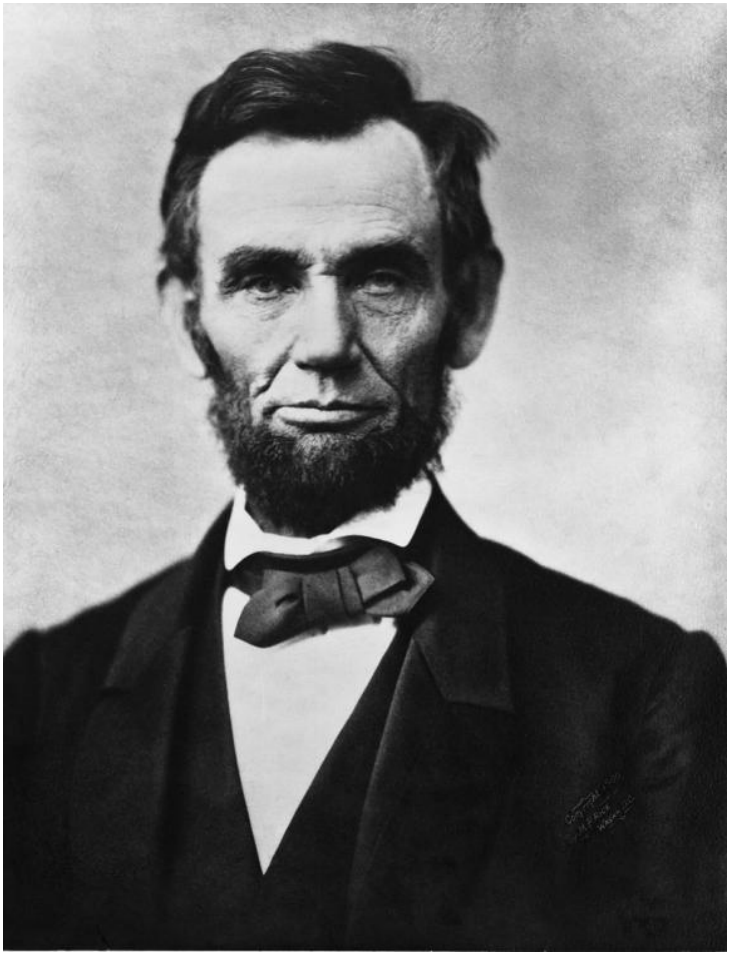
\includegraphics[width=\textwidth]{images/page_02_img_1.png}
  \end{column}
\end{columns}
\end{frame}

% Slide 3: Recap Data Mining Process
\begin{frame}{مرور: فرآیند داده‌کاوی}
  \centering
  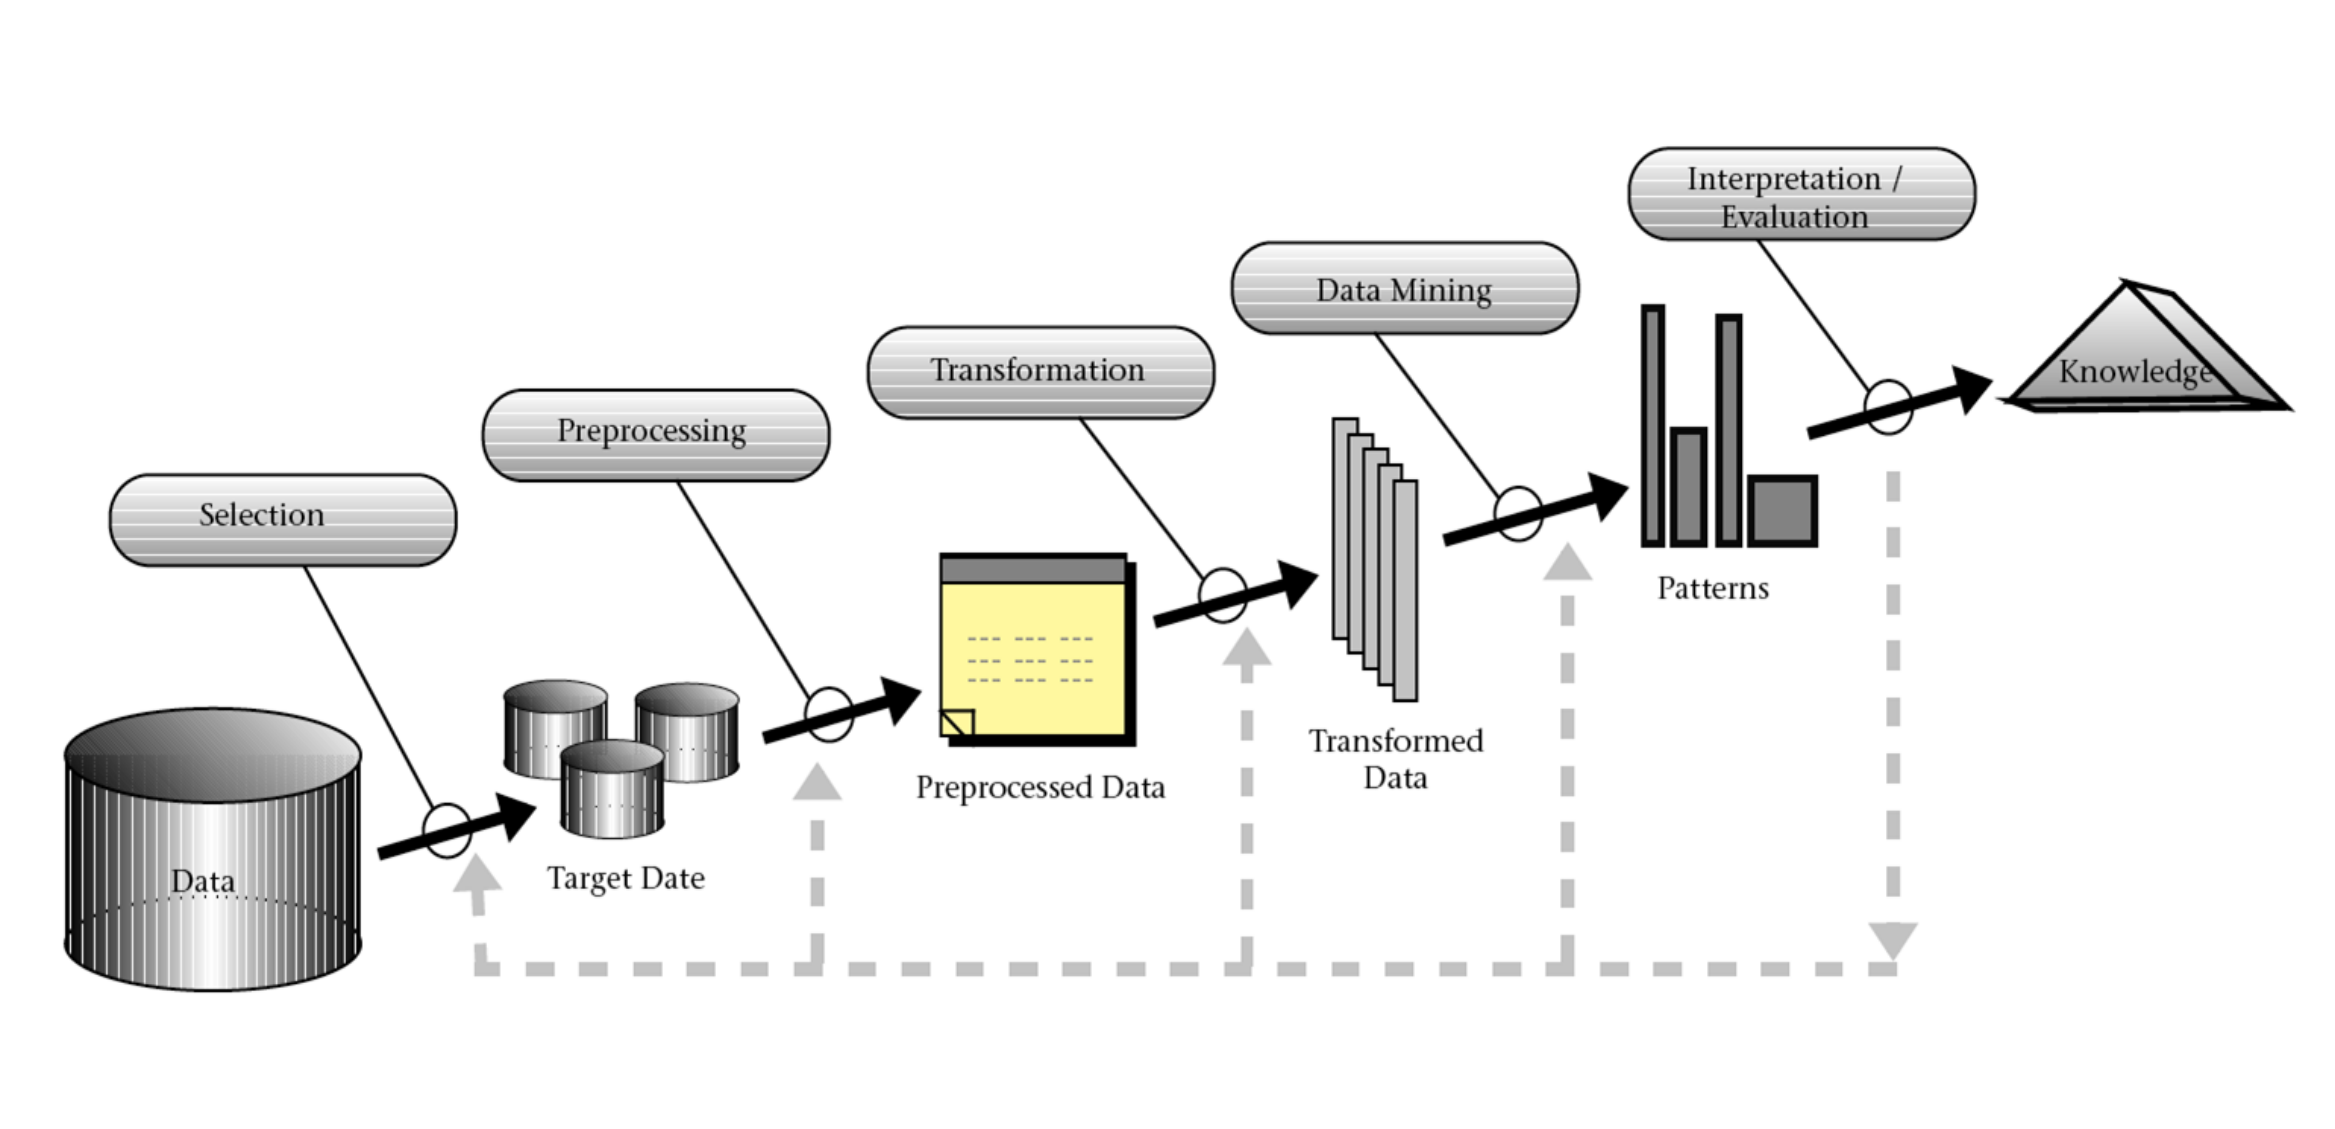
\includegraphics[width=0.96\textwidth]{images/page_03_img_1.png}
  \vspace{0.3cm}
  \flushright
  {\fontsize{7.5}{9}\selectfont\color{subgray}منبع: \lr{Fayyad et al. (1996)}}
\end{frame}

% Slide 4: Data Preprocessing
\begin{frame}{پیش‌پردازش داده‌ها}
\begin{columns}[c]
  \begin{column}{0.55\textwidth}
    \begin{itemize}
      \item \textbf{داده‌های شما ممکن است با مسائلی مواجه باشند:}
      \begin{itemize}
        \item به این معنی که ممکن است برای مراحل بعدی کاوش مشکل‌ساز شوند.
      \end{itemize}
      \vspace{0.3cm}
      \item پیش از ادامه و ورود به الگوریتم‌ها، این مسائل را برطرف کنید.
      \vspace{0.3cm}
      \item چه مسائلی به ذهنتان می‌رسد؟
    \end{itemize}
  \end{column}
  \begin{column}{0.42\textwidth}
    \centering
    
\includegraphics[width=\textwidth]{images/page_04_img_1.png}
  \end{column}
\end{columns}
\end{frame}

% Slide 5: Overview of Data Problems
\begin{frame}{پیش‌پردازش داده‌ها}
\begin{itemize}
  \item \textbf{مشکلاتی که ممکن است با داده‌های خود داشته باشید:}
  \begin{itemize}
    \item خطاها و داده‌های پرت (\lr{Errors \& Outliers})
    \item مقادیر گمشده / ازدست‌رفته (\lr{Missing Values})
    \item توزیع نامتوازن کلاس‌ها (\lr{Unbalanced Distribution})
    \item مقیاس‌های متفاوت ویژگی‌ها (\lr{Different Scales})
    \item متغیرهای پیش‌بینی کاذب / نشت داده (\lr{False Predictors})
    \item انواع داده‌های پشتیبانی‌نشده (\lr{Unsupported Data Types})
    \begin{itemize}
      \item داده‌های رسته‌ای/کیفی و تاریخ‌ها (\lr{Categorical Data \& Dates})
      \item مقادیر متنی (\lr{Textual Values})
    \end{itemize}
    \item ابعاد بالا / نفرین ابعاد (\lr{High Dimensionality})
    \begin{itemize}
      \item انتخاب زیرمجموعه ویژگی‌ها (\lr{Feature Subset Selection})
      \item تحلیل مؤلفه‌های اصلی (\lr{PCA})
      \item نمونه‌گیری (\lr{Sampling})
    \end{itemize}
  \end{itemize}
\end{itemize}
\end{frame}
